\nonstopmode

\documentclass[final,letterpaper,twoside,12pt]{article}

\usepackage[round, sort]{natbib}

\usepackage{graphicx}
\graphicspath{{Figures/}}


\usepackage{amsmath}

\usepackage{mathtools}

\usepackage{hyperref}

\title{Manual of the \texttt{MATLAB} pipeline for the analysis of genomic time course data from the \textit{Gene Expression Omnibus}}

\author{Juan Camilo Ram\'{i}rez}

\date{\today}

\begin{document}

\maketitle

\tableofcontents

\listoffigures

\listoftables

\section{Summary}

\begin{enumerate}

\item The pipeline analysis is performed individually for each experimental condition.

\item An experimental condition is composed of several GEO samples, all associated to a GEO series.

\item The information of each sample must be provided in an input file located in folder Input.

\item Several condition files can be deposited in folder Input and the pipeline analysis will be performed on all the conditions.

\item The analysis results for all condition files given as input are output in folder Results.

\item Section 1 explains how to prepare the condition files that will be given as input.

\item Section 2 explains how to run the analysis on the condition files created in Section 1. 

\end{enumerate}




\section{Theoretical basis and terminology}
\label{section:theory_and_terminology}

\subsection{Experimental conditions}

\subsection{Experimental macroconditions}

\subsection{Replicates}
\label{subsection:replicates_1}
\par Replicates can be \emph{biological} or \emph{technical}.\footnote{\href{https://honglangwang.wordpress.com/2012/04/24/【bio-glossary】biological-replicates-vs-technical-replicates/}{Biological Replicates vs Technical Replicates}.}

\subsection{Genes' between-replicate noise}
\label{subsection:replicates}
\par Genes may exhibit variation across replicates from the same condition. This variation, referred to as the \emph{gene's between-replicate noise} and denoted by $\delta$, is measured for each gene as follows. Let $x^s_{i,t}$ be the expression level of replicate $s$'s $i$-th gene at time $t$ and let $S$ be the total number of replicates. Let $\sigma_{i,t}$ be the standard deviation of the expression level of the $i$-th gene at time $t$ across the $S$ replicates. The gene $i$'s between-replicate noise, denoted by $\delta_i$,\footnote{Another possibility is to define $\delta_i$ in terms of the coefficient of variation instead of the standard deviation. In other words, the between-replicate noise could be defined as $\delta_i = \frac{1}{T} \sum_{t \in t_1}^{t_T} \frac{\sigma_{i,t}}{\mu_{i,t}}$, where $\mu_{i,t}$ is the mean of the expression level of the $i$-th gene at time $t$ across the $S$ replicates. However, this measure is unreliable given that expression levels are interval scale measures and the coefficient of variation is reliable only in ratio scale measures.} is given by

\begin{equation}
\label{equation:between_replicate_noise}
\delta_i = \frac{1}{T} \sum_{t \in t_1}^{t_T} \sigma_{i,t}.
\end{equation}

\par Section~\ref{section:between_replicate_noise_m} introduces the \texttt{MATLAB} function provided for the calculation of the genes' between-replicate noise from a group of replicates.

\section{The pipeline analysis}
\label{section:pipeline}


\section{Input files}
\label{section:input_files}

\subsection{Condition files}
\label{section:condition_files}

\par \emph{Condition files} are the input files for the pipeline analysis of one or more experimental conditions. The information of each experimental condition must be provided in a text file. One file for each condition. The condition files must be stored in folder \texttt{Input}. Each condition file must be named with the following format: \texttt{[GEO SERIES NUMBER]\_-\_[NAME OF EXPERIMENTAL CONDITION]\_-\_[NUMBER OF TOP DRGs FOR CLUSTERING].txt}.

\par All the samples associated with the experimental condition must be provided along with the time points using the format described as follows. Each line of the file must consist of the time point, including the time unit (e.g., 2 hours), followed by a comma (,) and then followed by the accession number of one sample. For example, the file for condition ``D10'' of \textit{GEO} series \texttt{GSE59015} must be named \texttt{GSE59015\_-\_D10\_-\_3000.csv} and the contents must be as follows.

\begin{center}
\begin{tabular}{ c }

0 hours,GSM1424453 \\
6 hours,GSM1424454 \\
12 hours,GSM1424455 \\
18 hours,GSM1424456 \\
24 hours,GSM1424457 \\
30 hours,GSM1424458 \\
36 hours,GSM1424459 \\
42 hours,GSM1424460 \\

\end{tabular}
\end{center}

\par The condition file can group different replicates that represent the same experimental condition. In this case the pipeline will run one single analysis with the average of all the replicates specified in the file. For example, the file for all the replicates in \textit{GEO} series \texttt{GSE41067} must be named \texttt{GSE41067\_-\_ALL\_-\_10000.csv} and the contents must be as follows.

\begin{center}
\begin{tabular}{ c }

0 hours,GSM1008154,GSM1008162,GSM1008170 \\
1 hours,GSM1008155,GSM1008163,GSM1008171 \\
2 hours,GSM1008156,GSM1008164,GSM1008172 \\
4 hours,GSM1008157,GSM1008165,GSM1008173 \\
6 hours,GSM1008158,GSM1008166,GSM1008174 \\
8 hours,GSM1008159,GSM1008167,GSM1008175 \\
10 hours,GSM1008160,GSM1008168,GSM1008176 \\
12 hours,GSM1008161,GSM1008169,GSM1008177 \\


\end{tabular}
\end{center}

\par The condition files can be written manually, following strictly the format described above. Optionally, this task can be carried out more easily by using script \texttt{create\_input\_files.m}. In order to do this, \texttt{create\_input\_files.m} must be run and the instructions provided thereafter by the program must be followed. More details in Section~\ref{section:user_functions}.

\subsection{Macrocondition files}
\label{subsection:macrocondition}

\par The conditions comprising the macrocondition must be provided in a text file that must be located in folder \texttt{Input}. This file must be named using the following format: \texttt{[GEO SERIES NUMBER]\_-\_[NAME OF MACRO CONDITION].txt}. For example, the following are the contents of a macrocondition of five H3N1 subjects from \texttt{GSE52428}.

\begin{center}
\begin{tabular}{ c }

H3N1\_001 \\
H3N1\_002 \\
H3N1\_003 \\
H3N1\_004 \\
H3N1\_005 \\

\end{tabular}
\end{center}


\par This file can be constructed manually, or with BASH script \texttt{prepare\_input.sh}. This option requires running the script with the following syntax.

\texttt{./prepare\_input.sh [GEO SERIES] [NAME OF MACRO CONDITION].txt}

\par Example

\texttt{./prepare\_input.sh GSE52428 H1N1.txt}

\par The above will read ALL the conditions whose analyses have been completed for the GEO series indicated and write the file with the format described earlier.

\section{\texttt{create\_input\_files.m}}
\label{section:user_functions}

\par The (experimental) condition files for the pipeline analysis can be created manually with the format described in Section~\ref{section:condition_files} or with the help of script \texttt{create\_input\_files.m}. In order to do the latter, the command \texttt{create\_input\_files} must be executed on the \texttt{MATLAB} console from the pipeline directory, as shown in Figure~\ref{figure:create_files}.

\iffalse
\begin{figure}[h]
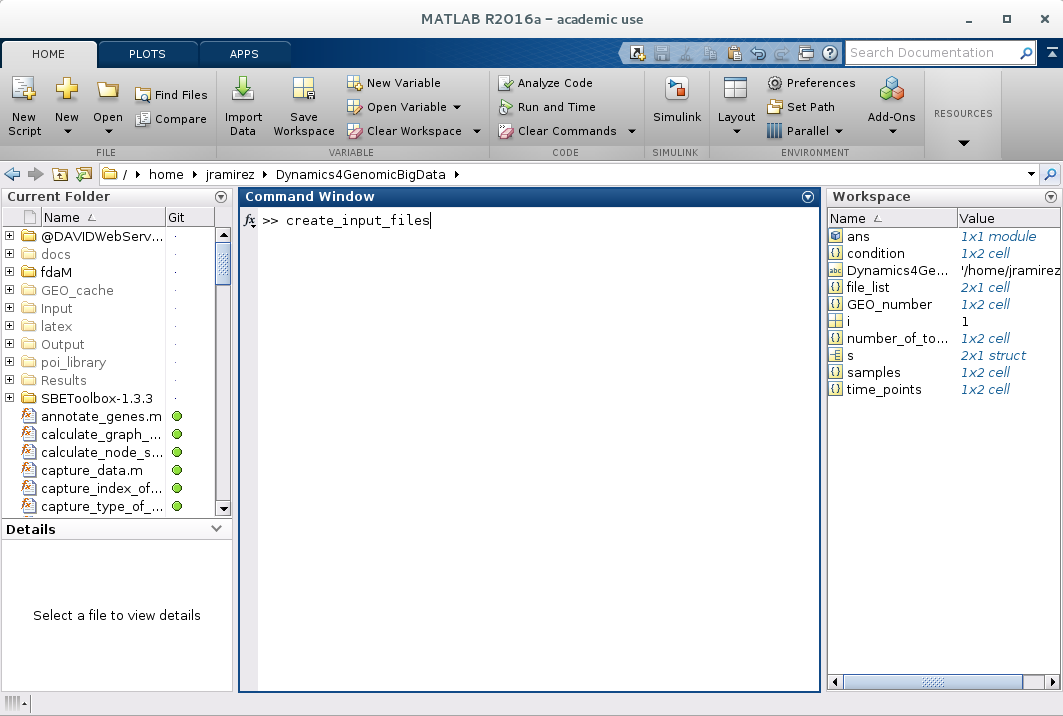
\includegraphics[width=\textwidth]{create_files}
\caption{Executing the \texttt{create\_input\_files.m} script in order to create the condition file(s) to be used in the pipeline analysis.}
\label{figure:create_files}
\end{figure}


\begin{figure}[h]
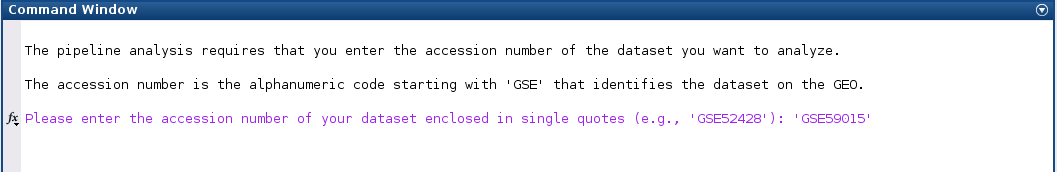
\includegraphics[width=\textwidth]{create_files_2}
\caption{Executing the \texttt{create\_input\_files.m} script in order to create the condition file(s) to be used in the pipeline analysis.}
\label{figure:create_files_2}
\end{figure}

\begin{figure}[h]
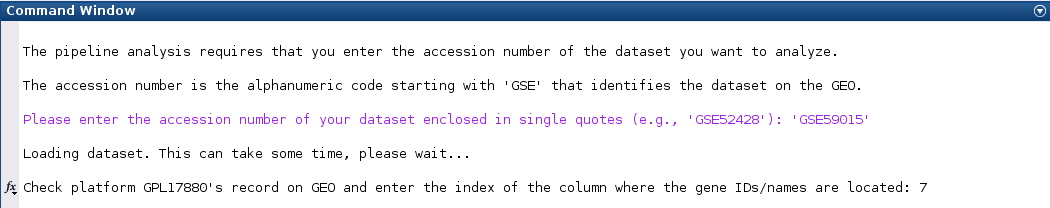
\includegraphics[width=\textwidth]{create_files_3}
\caption{Executing the \texttt{create\_input\_files.m} script in order to create the condition file(s) to be used in the pipeline analysis.}
\label{figure:create_files_3}
\end{figure}

\begin{figure}[h]
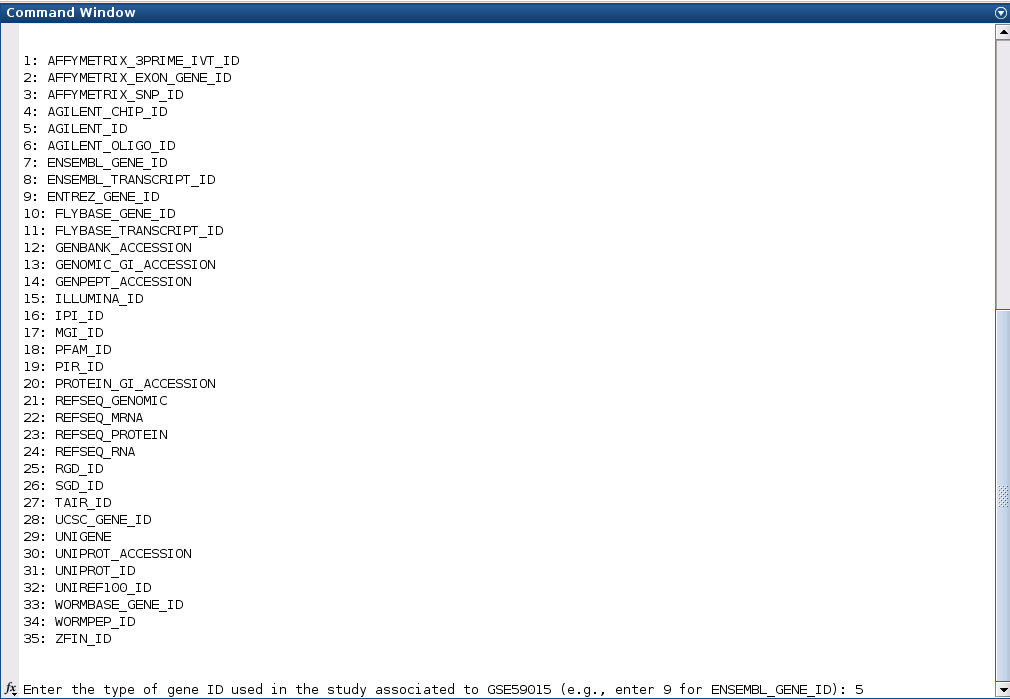
\includegraphics[width=\textwidth]{create_files_4}
\caption{Executing the \texttt{create\_input\_files.m} script in order to create the condition file(s) to be used in the pipeline analysis.}
\label{figure:create_files_4}
\end{figure}

\begin{figure}[h]
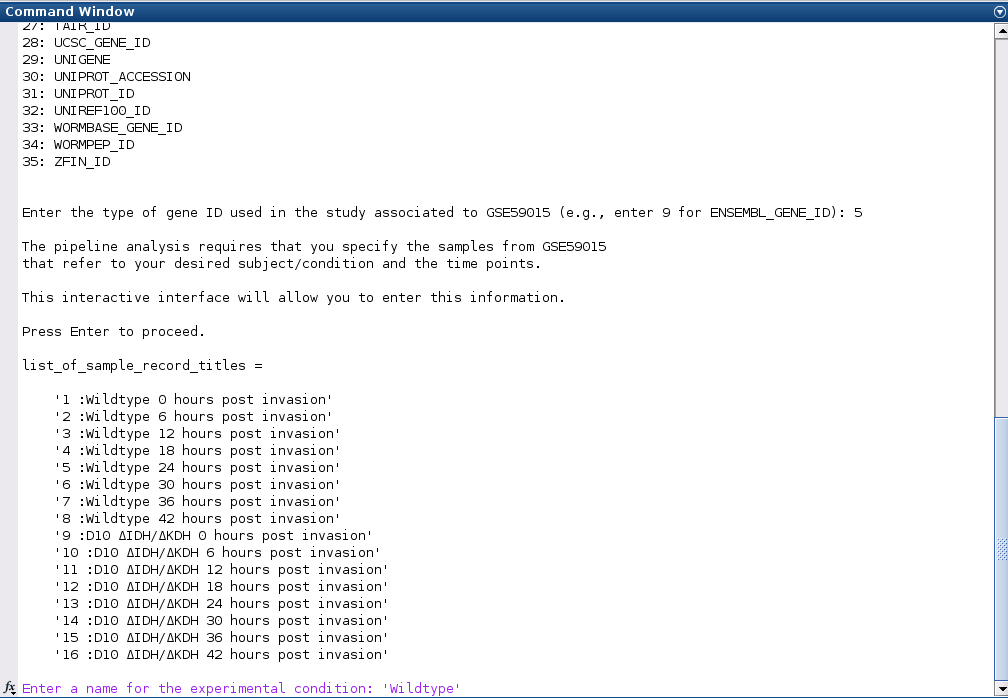
\includegraphics[width=\textwidth]{create_files_5}
\caption{Executing the \texttt{create\_input\_files.m} script in order to create the condition file(s) to be used in the pipeline analysis.}
\label{figure:create_files_5}
\end{figure}

\begin{figure}[h]
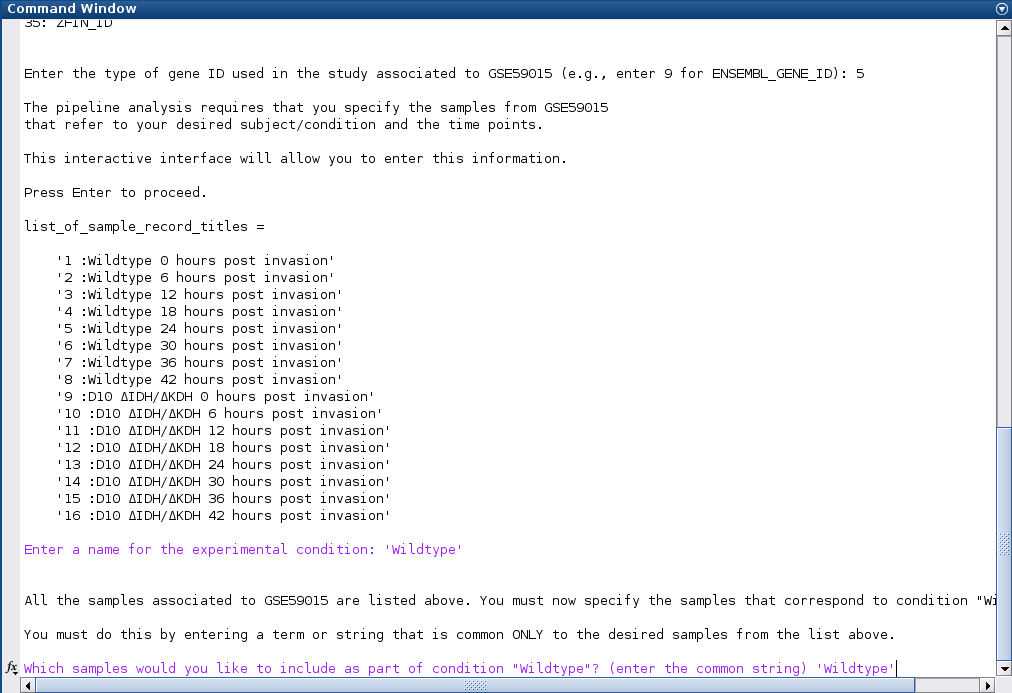
\includegraphics[width=\textwidth]{create_files_6}
\caption{Executing the \texttt{create\_input\_files.m} script in order to create the condition file(s) to be used in the pipeline analysis.}
\label{figure:create_files_6}
\end{figure}

\begin{figure}[h]
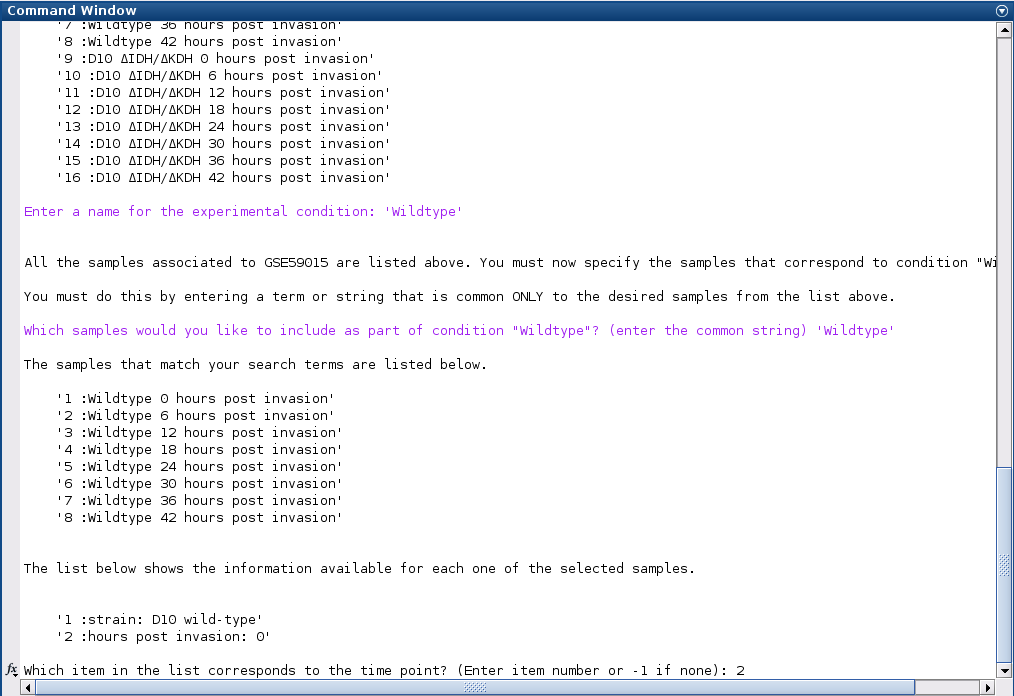
\includegraphics[width=\textwidth]{create_files_7}
\caption{Executing the \texttt{create\_input\_files.m} script in order to create the condition file(s) to be used in the pipeline analysis.}
\label{figure:create_files_7}
\end{figure}

\begin{figure}[h]
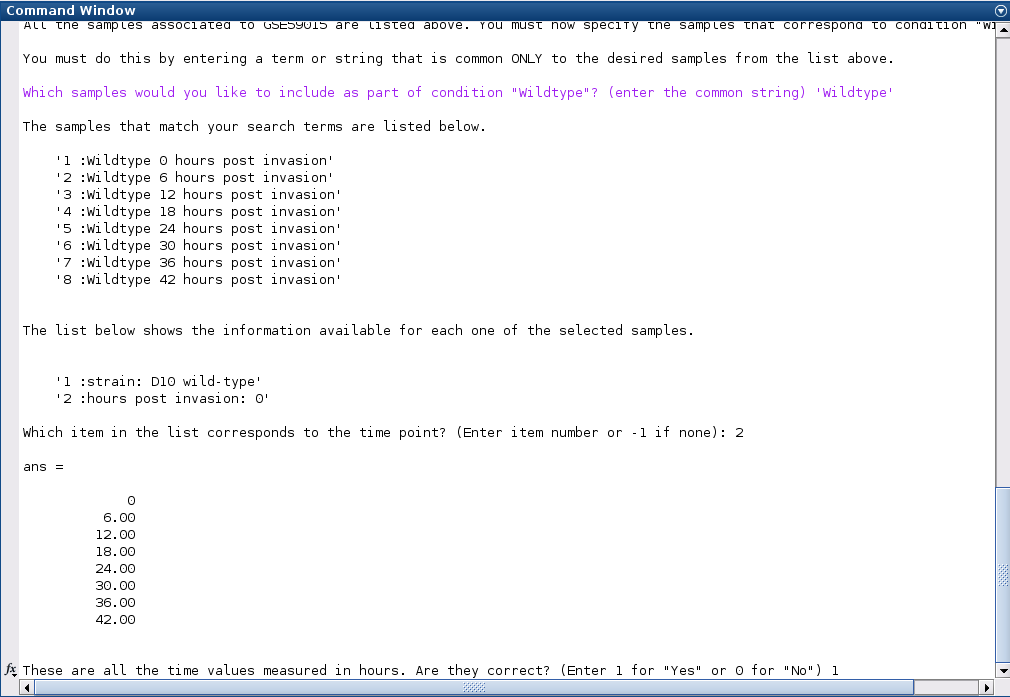
\includegraphics[width=\textwidth]{create_files_8}
\caption{Executing the \texttt{create\_input\_files.m} script in order to create the condition file(s) to be used in the pipeline analysis.}
\label{figure:create_files_8}
\end{figure}

\begin{figure}[h]
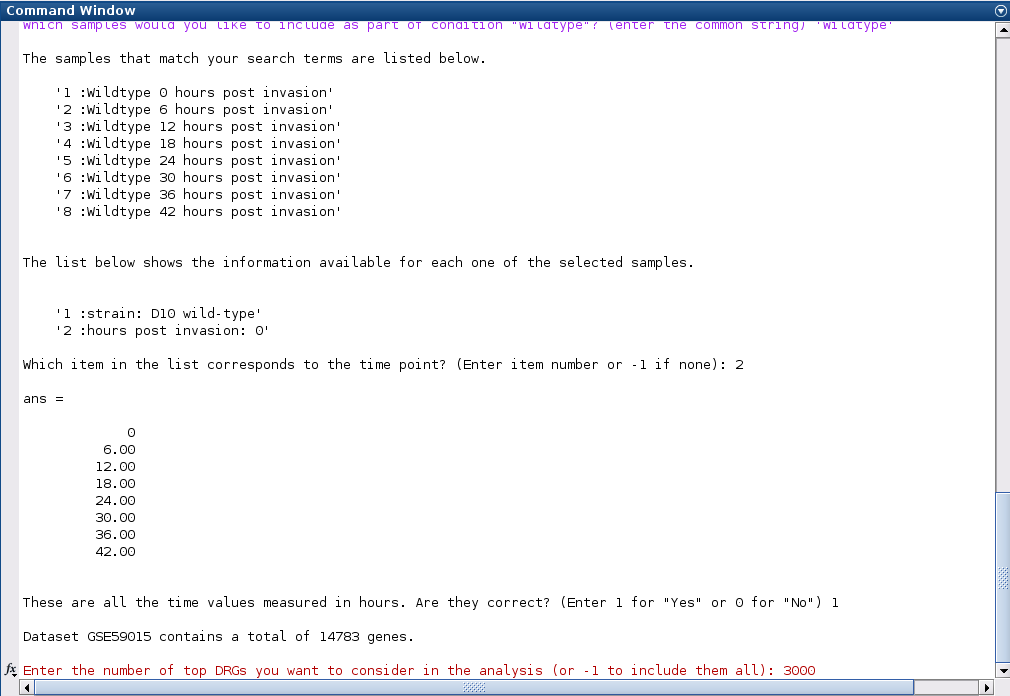
\includegraphics[width=\textwidth]{create_files_9}
\caption{Executing the \texttt{create\_input\_files.m} script in order to create the condition file(s) to be used in the pipeline analysis.}
\label{figure:create_files_9}
\end{figure}

\begin{figure}[h]
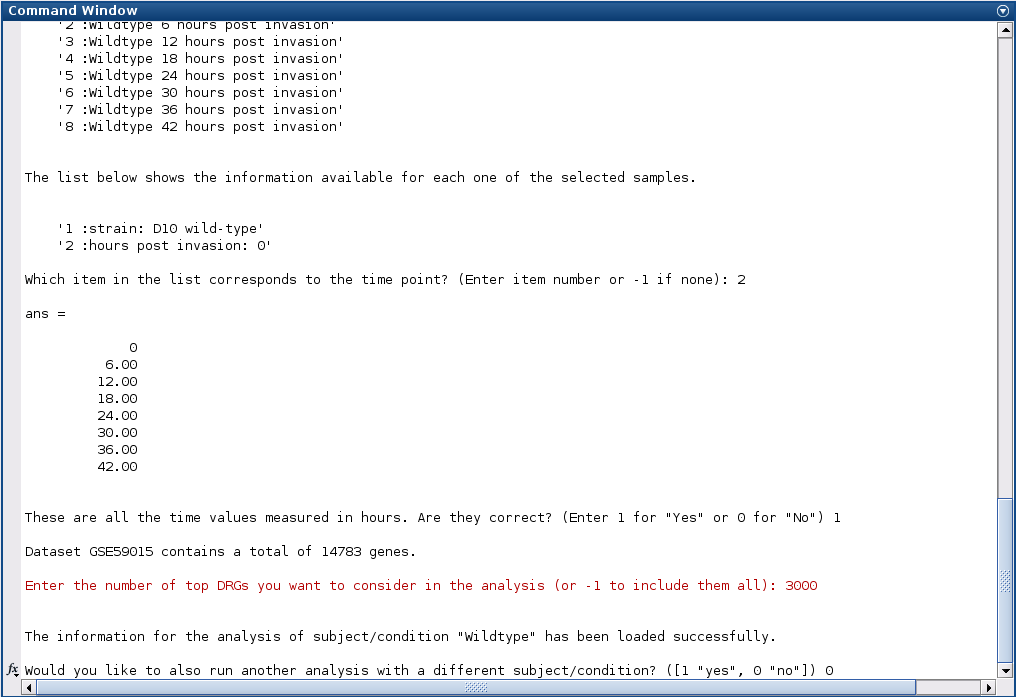
\includegraphics[width=\textwidth]{create_files_10}
\caption{Executing the \texttt{create\_input\_files.m} script in order to create the condition file(s) to be used in the pipeline analysis.}
\label{figure:create_files_10}
\end{figure}

\begin{figure}[h]
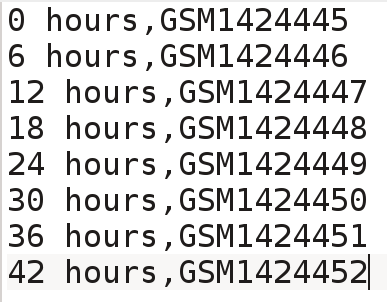
\includegraphics[width=\textwidth]{create_files_11}
\caption{Executing the \texttt{create\_input\_files.m} script in order to create the condition file(s) to be used in the pipeline analysis.}
\label{figure:create_files_11}
\end{figure}

\section{\texttt{pipeline.m}}

\par The condition files must be prepared, as described in Section~\ref{section:condition_files}, and placed in folder \texttt{Input}. After this, the pipeline analysis can be started by opening the \texttt{MATLAB} console in the pipeline directory and running \texttt{pipeline}, as shown in Figure~\ref{figure:pipeline1}

\begin{figure}[h]
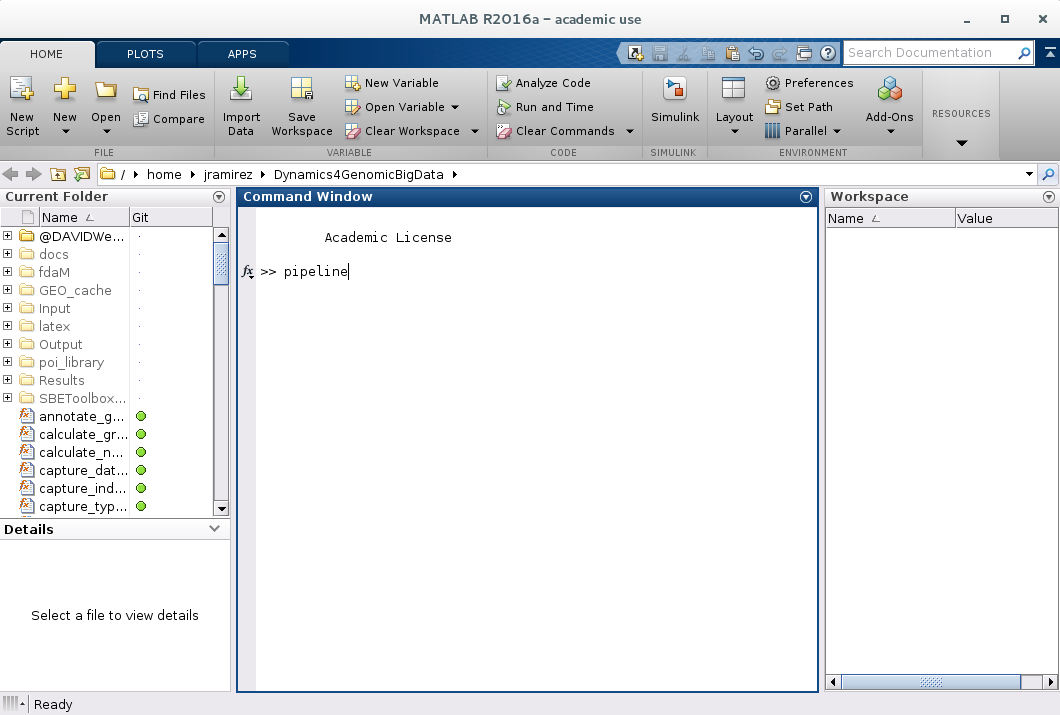
\includegraphics[width=\textwidth]{pln1}
\caption{Executing the \texttt{pipeline.m} script in order to run the pipeline analysis on a set of one or more experimental conditions.}
\label{figure:pipeline1}
\end{figure}

\fi

\par Once all condition files are located in folder Input, then the analysis can be started by running pipeline.m. The script will read ALL the condition files in folder Input and run the analysis for each one of them.

\section{\texttt{integrated\_analisis.m}}

\par \texttt{integrated\_analisis.m}: input is a macrocondition file. See Subsection~\ref{subsection:macrocondition}.

\section{\texttt{compare.m}}

\par \texttt{compare.m}: input is a macrocondition file. See Subsection~\ref{subsection:macrocondition}.

\section{\texttt{measure\_fit\_of\_replicates.m}}
\label{section:between_replicate_noise_m}

\par This is a script that calculates the between-replicate noise for all genes across a number of replicates, as shown in Subsection~\ref{subsection:replicates}. Its input is a macrocondition file, as defined in Subsection~\ref{subsection:macrocondition}. Results will be output in folder \texttt{Pipeline\_HOME/Output/[GSE Series]/Comparison\_of\_replicates/[Macrocondition]/}.

\par This folder contains a file named \texttt{[Macrocondition]\_noise\_per\_gene\_ALL\_GENES.csv}. Each line of this file corresponds to a probe in the GSE matrix and contains three values separated by commas (,). The first field is the probe ID, the second is the gene name, and the third is the gene's between-replicate noise. The probes are listed in this file in the same order they appear in the GSE matrix. A secondary file, named \texttt{[Macrocondition]\_noise\_per\_gene\_ALL\_GENES\_SORTED\_BY\_NOISE.csv}, provides the same information with the probes listed by their between-replicate noise in decreasing order. That is to say, probes that appear on top are the ones whose expression is most consistent across the probes provided in the macrocondition file whereas those at the bottom are the ones exhibiting the most discrepancy in expression across these replicates.



\bibliographystyle{myapalike}
\bibliography{bibliography}
\end{document}

